\documentclass{article}
\usepackage[margin=24mm]{geometry}
\usepackage{tikz}
\setlength{\emergencystretch}{3em}
\title{Matroid inverse: decoder integration audit}
\date{Created-at: 2026-10-29 00:29 CET}
\begin{document}\maketitle
\paragraph{Goal and acceptance.} Audit the complete 883-qubit decoder's inverse
interfaces and live workspace. Compile an explicitly initialized-output inverse
from the existing canonical arithmetic model, verify its measured cleanup,
compose its zero flag, and compare complete jet costs. Only a promising verified
candidate proceeds to the official 102400-shot fixed-salt evaluation. A rejected
candidate with exact reasons is a valid campaign outcome; no improvement promised.
\paragraph{Ownership.} Transformation/Quantum owns arithmetic contracts,
certificates and native composition. Core retains the authored model and Graph
supplies existing checked matroid witnesses. The external Apache generator owns
its kernels; its snapshot remains read-only. No provider changes, new dependencies,
publication, WSL or duplicate checkouts. Continue existing dirty task paths only.
\paragraph{Changes.} Extend synthesis/arithmetic.rs, Python arithmetic.py and
reversible.py, arithmetic data/source and tests; extend hermite.py and its Kaggle
CLI/tests for immutable composition and audit; extend quantum inverse preparation
and report.py. Artifacts: canonical projection, source identities, native receipts,
cost table, figure/PDF and continuation. Protected CORE.YAML items: empty.
\paragraph{Contract.} Preserve the arbitrary-target XOR inverse. Add an explicit
initialized-output specialization whose scratch equals Norm(output). Certify all
64 inputs and all eight measurement masks against the retained reference prefix.
The native adapter refuses this specialization at arbitrary-target call sites.
Zero flag is computed from the live three-bit inverse norm before its erasure;
check its value and phase, including input zero. Basis changes are checked against
the independent native GF(64) embedding. No source names imply semantics.
\paragraph{Integration.} Rebind public functions through their existing bind
facade, including recursive cached inverse and reverse start-inverse; never mutate
module globals. Count local peak including outputs/flag, retained allocation,
Toffolis, and full jet pairs with 840 live qubits. Reuse previously verified call
counts and incumbent score for explicitly conditional estimates. A complete
decoder score is reported only after an actual full official run.
\paragraph{Verification.} Targeted Rust arithmetic tests; Python contract,
aliasing, basis and cost tests. Native all 64 fresh inputs at three measurement
seeds, arbitrary-target regression at 4096 inputs, diagonal phase probes and
round-trip jet checks including zero and boundaries. Serialize/reload small native
artifacts. Compare the public fresh inverse under the same contract.
\paragraph{Budget and ETA.} Approximately 60--90 minutes: implementation and
exact checks, bounded native cells, decision/report/archive. One CPU, 2 GiB and
900 seconds for small cells; only an admitted full candidate may use 12 GiB and
900 seconds per build/verify. Native Python on Amaterasu; 317 GiB home free at
start. Execute current Python source in memory from stdin, with read-only existing
runtime and public snapshot mounts; no new remote source tree. Local target reused.
\paragraph{Risks and rollback.} Zero-only cleanup is invalid for arbitrary
targets; missing flag, basis conversion or deferred phase breaks composition.
An isolated Q-squared-T gain can regress globally when 840 qubits stay live.
Reject regressions before full verification. Preserve incumbent, unrelated edits
and old evidence; rollback only named task changes. No global optimality or RL claim.
\begin{center}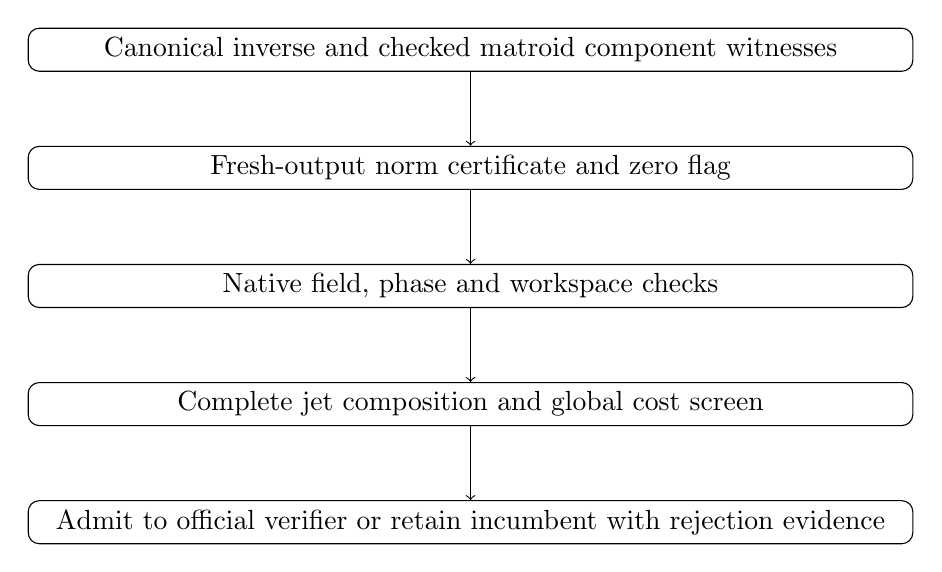
\begin{tikzpicture}[every node/.style={draw,rounded corners,align=center,text width=11cm},node distance=15mm]
\node (a) {Canonical inverse and checked matroid component witnesses};
\node (b) [below of=a] {Fresh-output norm certificate and zero flag};
\node (c) [below of=b] {Native field, phase and workspace checks};
\node (d) [below of=c] {Complete jet composition and global cost screen};
\node (e) [below of=d] {Admit to official verifier or retain incumbent with rejection evidence};
\draw[->] (a)--(b);\draw[->] (b)--(c);\draw[->] (c)--(d);\draw[->] (d)--(e);
\end{tikzpicture}
\end{center}
\end{document}
